\documentclass[a4paper,10pt,headlines=3.2]{scrartcl}
\usepackage{graphicx}           %Bilder

%\usepackage[T1]{fontenc}        %Umlaute
%\usepackage[latin1]{inputenc}   %Windows
%\usepackage[utf8x]{inputenc}	%Linux
\usepackage{ucs}

\usepackage[ngerman]{babel}     %Deutsche Sprache
\usepackage{amsmath}            %Math. Zeichen
\usepackage{pifont}             %Skalierbare Schriftart
\usepackage{array}
\usepackage{epsfig}             %Erweiterte Grafiken
\usepackage{makeidx}            %Stichwortverzeichnis
\usepackage[pdftex]{color} 

\newcommand{\changefont}[3]{
\fontfamily{#1} \fontseries{#2} \fontshape{#3} \selectfont}

\makeindex

\usepackage[automark]{scrpage2}
\usepackage[nosectionbib]{apacite}               %Zitieren

%\usepackage[colorlinks]{hyperref}%Hyperlinks

\usepackage{lmodern}
\usepackage{scrpage2}           %KOMA-Script
\usepackage{tipa}
\usepackage{qtree}
\usepackage{pgf}


\usepackage{remreset}			%Fussnoten global
\makeatletter
\@removefromreset{footnote}{chapter}
\makeatother 

\setcounter{tocdepth}{3}

%Kopfzeilen
\pagestyle{scrheadings}         %Seitenstil scrheadings verwenden

%\setlength{\textheight}{24cm}
%\setlength{\textwidth}{16cm}
%\setlength{\topmargin}{-2cm}
%\setlength{\oddsidemargin}{0cm}

% Groesse des Textbereiches in der Seite
\setlength{\textwidth}{16cm}
\setlength{\textheight}{22cm}
% Kopf- und Fusszeile, Hoehe und Abstand vom Text
\setlength{\headheight}{15pt}
\setlength{\headsep}{0.8cm}
% Linker Seiteneinzug
\setlength{\oddsidemargin}{2.5cm} \addtolength{\oddsidemargin}{-1in}
\setlength{\evensidemargin}{2.5cm} \addtolength{\evensidemargin}{-1in}
% Andere Groessen ausrechnen (vertikal zentrieren)
\setlength{\footskip}{\headsep}
\addtolength{\footskip}{\headheight}
\setlength{\topmargin}{\paperheight}
\addtolength{\topmargin}{-\textheight}
\addtolength{\topmargin}{-\headheight}
\addtolength{\topmargin}{-\headsep}
\addtolength{\topmargin}{-\footskip}
\addtolength{\topmargin}{-2in}
\addtolength{\topmargin}{-0.5\topmargin}

%Schriftart
\changefont{cmss}{m}{n}

%Abstand zur�cksetzen
\setlength{\headheight}{20pt}

\usepackage{listings} 
\lstset{numbers=left, numberstyle=\tiny, numbersep=5pt} \lstset{language=Java} 

\clearscrheadfoot
%\renewcommand{\headheight}{40pt} 
\ihead[]{Datenstrukturen und Algorithmen \\Fr�hlingssemester 2011 \\Institut f�r angewandte Mathematik} % - links
\ohead[asdasd]{�bungsblatt 4 \\Abgabetermin 24. M�rz 2011 \\Adrianus Kleemans [07-111-693]} % - linke Kopfzeile 
\setheadsepline{.4pt} %Separate Linie im Kopf
\cfoot[\pagemark]{\pagemark} %- mittlere Fusszeile 

\begin{document}
\section*{Theoretische Aufgaben}
\subsection*{Aufgabe 1}
Der CountingSort-Algorithmus ist relativ leicht zu erkl�ren, dies kann in 4 
Schleifen geschehen:
\begin{enumerate}
 \item Die erste Schleife stellt ein leeres Feld C bereit, von 0 bis zur h�chsten vorkommenden Zahl.
 \item Die zweite Schleife z�hlt iterierend, wieviel mal j vorkommt und speichert dies in $C[j]$.
 \item Die dritte Schleife z�hlt die f�r die Elemente 0 bis i von C fortlaufend zusammen und speichert den Wert bei
jedem Durchgang in $C[i]$.
 \item Die vierte Schleife nimmt den obersten Wert von der Eingabe A, setzt ihn als Index in C ein. Dort steht der Index
von B, wo der oberste Wert von A abgespeichert werden soll. Dies wiederholt sich, bis alle Elemente eingef�gt
wurden.
\end{enumerate}

\begin{figure}[ht]
\centering
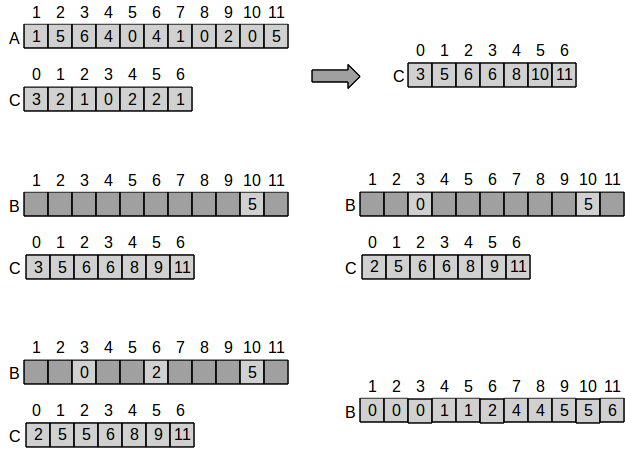
\includegraphics[height=6cm]{aufg1}
\end{figure}

\subsection*{Aufgabe 2}
\lstset{frame=single}
\begin{lstlisting}[caption=Aufgabe 2]{Name}
// bereitet die Abfrage vor
void prepare(A, k)
int C[k]
for i = 0 to k
  C[i] = 0
for j = 1 to A.length
  C[A[j]] = C[A[j]] + 1
for i = 1 to k
  C[i] = C[i] + C[i - 1]

// Abfrage
int query(a, b)
if a = 0
  return C[b]
else
  return C[b] - C[a-1]
\end{lstlisting}

\subsection*{Aufgabe 3}
Die einzelnen Elemente werden mit dem hintersten Buchstaben beginnend buchstabenweise sortiert. Das heisst, es wird
zuerst bei allen der hinterste, dann der mittlere, und zum Schluss nach dem vordersten Buchstaben sortiert.

\begin{figure}[ht]
\centering
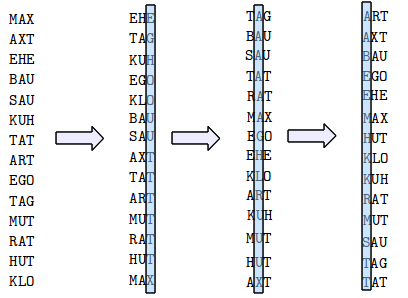
\includegraphics[height=7cm]{aufg3}
\end{figure}

\subsection*{Aufgabe 4}
Stabilit�t der Sortieralgorithmen:
\begin{itemize}
 \item InsertionSort: Ja. Elemente werden nicht mehr ausgeatuscht, wenn n�chstvorderes Element gleichgross ist.
 \item MergeSort: Ja. bei gleichen Elementen wird zuerst aus dem ersten Array das (urspr�nglich vordere) Element
eingesetzt, somit wird die Reihenfolge erhalten.
 \item HeapSort: Nein. Aufgrund der Verteilung auf verschiedene Teilb�ume kommt es auf die anderen Zahlen an, ob zwei
gleiche Elemente vertauscht werden oder nicht.
 \item QuickSort: Nein. Durch den Austausch rund um die fortschreitende Z�hlvariable (und wo bestimmt
wird, ob die folgende Zahl gr�sser oder kleiner dem Pivot ist) werden die Elemente so 'herumgeschoben', dass es nach
einem Durchlauf m�glich ist, dass zwei gleiche Elemente in umgekehrter Reihenfolge anzutreffen sind.
\end{itemize}

\subsection*{Aufgabe 5}
\begin{figure}[ht]
\centering
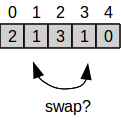
\includegraphics[height=2cm]{aufg5}
\end{figure}
Bei einem Austausch kann bei Elementen zus�tzlich noch der Index selbst verwendet werden, um sicherzustellen, dass der
Algorithmus stabil l�uft. Dabei wird bei einem Vergleich ein einfacher Test $i_{1} < i_{2}$ gemacht, um zu verhindern,
dass ein \texttt{swap} mit gleichen Elementen stattfindet.

\subsection*{Aufgabe 6}
Angenommen, es gibt unter den Zahlen $k$ unterschiedliche L�ngen. F�r jede L�nge $k_{x}$ gilt, dass sie zuerst sortiert
werden muss, und die verschiedenen Teilergebnisse f�r die L�ngen $k_{1, 2, 3, ...}$ k�nnen dann aneinandergereiht
werden. Die Sortierdauer f�r alle Elemente der L�nge $k$ dauert der Sortiervorgang $\frac{n}{k_{1}}$.\\
Zusammengez�hlt ergeben die Laufzeiten f�r die verschieden langen Elemente die Gesamtlaufzeit:\\
\begin{eqnarray}
O\left(\frac{n}{k_{1}}\right) + O\left(\frac{n}{k_{2}}\right) + O\left(\frac{n}{k_{3}}\right) + \cdots +
O\left(\frac{n}{k_{n}}\right)\\
\Rightarrow O\left(\frac{n}{k_{1} + k_{2} + \cdots + k_{n}}\right)\\
\Rightarrow O\left(\frac{n}{1}\right) = O(n)
\end{eqnarray}

\section*{Praktische Aufgaben}
\subsection*{Aufgabe 1}
�ussere Schleife: $\Theta(d)$. Innere Schleife: $n\cdot\Theta(1)$. Gesamter Algorithmus: $\Theta(d*n)$
\subsection*{Aufgabe 2}
Siehe Beilagen \texttt{RadixSort.Java, RadixMiniTest.out, RadixSortTester.out}.

\subsection*{Aufgabe 3}
\begin{figure}[ht]
\centering
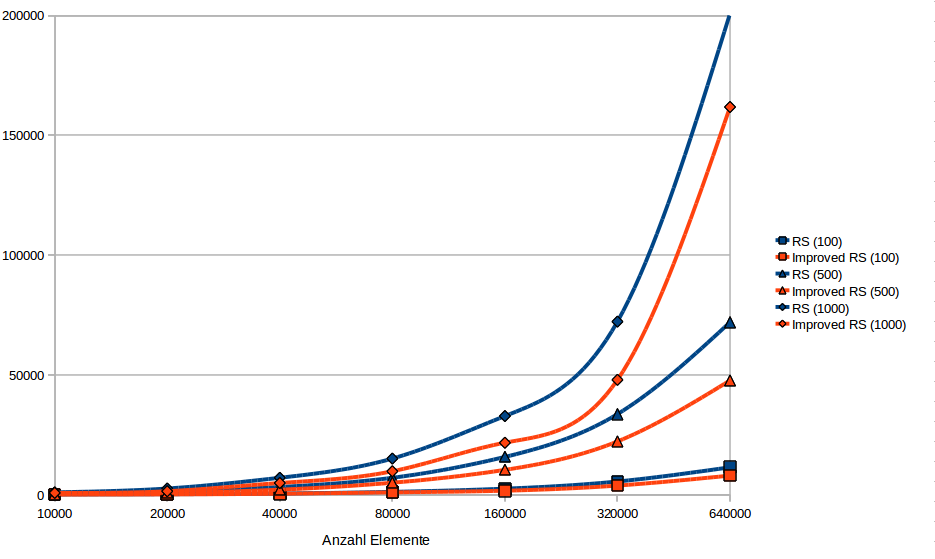
\includegraphics[height=8cm]{aufgt3}
\end{figure}
Die Parameter in der Grafik geben geben den Wert von $d$ aus, der auf 100, 500 und 1000 eingegeben wurde.\\
Die Laufzeit ist um 20-30\% verbessert worden (siehe \texttt{RadixSortTester.out} f�r die exakten Laufzeiten), scheint
jedoch noch nicht linear zu sein, sondern um einen Faktor kleiner als die Zeit f�r den 'normalen' radixSort. Evtl.
spielen auch die gew�hlten Datenstrukturen eine Rolle, welche noch optimaler gew�hlt werden k�nnten.

\end{document}